\section{Introduzione}\label{sec:introduzione}
\normalsize
Il mondo dei videogiochi ha subito una rapida evoluzione negli ultimi anni, arrivando al punto che alcuni di questi possono essere già definiti come dei veri e propri Esports. Questo sviluppo ha contribuito a rendere questo settore sempre piu` competitivo e dinamico.\\*\par
I giochi multiplayer spesso dividono i giocatori in leghe o gradi in modo tale da rendere le partite bilanciate, ovvero affinché ogni giocatore trovi un avversario che abbia un livello simile al suo. Per implementare questa soluzione sono solitamente usati dei sistemi a punti che premiano le vittorie e puniscono le sconfitte.
Tutto ciò però non è spesso sufficiente a garantire il bilanciamento dei giochi, la prova di questo penso si possa trovare nel fenomeno detto smurfing, che sta spopolando in molti giochi, forse l'esempio più lampante si può trovare in Leagues of legends, dove perfino la casa produttrice si è trovata costretta a prendere misure a riguardo, come si può leggere nell'articolo scritto da Outplayed sul tema\cite{Outplayed}, ma comunque è pratica che sta diventando comune in diversi titoli videoludici.
\\*\\*
Lo smurfing consiste nel creare un nuovo account con lo scopo di nascondere la reale identità del giocatore e usarlo al posto dell'account reale.\\*
Le ragioni dietro questa pratica possono essere molteplici: da giocatori professionisti che vogliono usare un altro account per fare pratica e nascondere le proprie strategie, al comportamento ben più nocivo del “newb bashing”, ovvero giocatori di livello medio-alto che si fanno un nuovo account per giocare contro i principianti e sembrare quindi dei fuoriclasse durante le partite. \\*\par
Attraverso questo report cercherò di capire se esiste un metodo per dividere i giocatori in leghe migliore rispetto ai sistemi a punti o quantomeno che possa integrarsi ad essi per migliorarli.\\*\\*
Il videogioco su cui baserò la mia ricerca è StarCraft II, un gioco di strategia in tempo reale a tema fantascientifico nonché uno dei principali Esports. Starcraft II usa un sistema a punti per dividere i giocatori in 7 diversi rank dal piu` basso al piu` alto: Bronzo, Argento, Oro, Platino, Diamante, Master e Grand Master. Oltre a questi è stato aggiunto al dataset anche un ottavo rank, quello dei giocatori professionisti:
questa modifica è stata effettuata perché non tutti i giocatori a Grand Master sono abbastanza forti per competere nei tornei più importanti. 
\begin{figure}[h]
	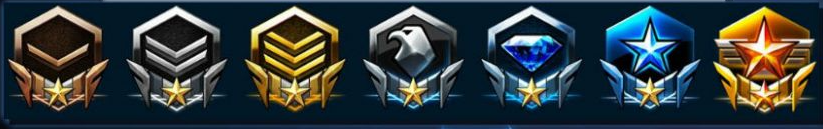
\includegraphics[scale=0.74]{../figures/ranks starcraft II.PNG}
	\caption{Leghe di Starcraft} 
\end{figure}
